

% DelPrete packages

\chapter{Robustness to Inertial Parameter Errors for Legged Robots Balancing on Level Ground}

% \section{Abstract}
% Model-based control  has become more and more popular in the legged robots community in the last ten years. 
% The key idea is to exploit a model of the system to compute precise motor commands that result in the desired motion.
% This allows to improve the quality of the motion tracking, while using lower gains, leading so to higher compliance.
% However, the main flaw of this approach is typically its lack of robustness to modeling errors.
% In this paper we focus on the robustness of inverse-dynamics control to errors in the inertial parameters of the robot.
% We assume these parameters to be known, but only with a certain accuracy.
% We then propose a computationally-efficient optimization-based controller that ensures the balance of the robot despite these uncertainties.
% We used the proposed controller in simulation to perform different reaching tasks with the HRP-2 humanoid robot, in the presence of various modeling errors.
% Comparisons against a standard inverse-dynamics controller through hundreds of simulations show the superiority of the proposed controller in ensuring the robot balance.


Model-based control has become more and more popular in the legged robots community in the last ten years. 
The key idea is to exploit a model of the system to compute precise motor commands that result in the desired motion.
This allows to improve the quality of the motion tracking, while using lower gains, leading so to higher compliance.
However, the main flaw of this approach is typically its lack of robustness to modeling errors. In this chapter we focus on the robustness of inverse-dynamics control to errors in the inertial parameters of the robot. We assume these parameters to be known, but only with a certain accuracy. We then propose a computationally-efficient optimization-based controller that ensures the balance of the robot despite these uncertainties. We used the proposed controller in simulation to perform different reaching tasks with the HRP-2 humanoid robot, in the presence of various modeling errors.Comparisons against a standard inverse-dynamics controller through hundreds of simulations show the superiority of the proposed controller in ensuring the robot balance.
\section{Introduction}
The problem of balancing for real legged robots is still a challenge for the robotics community.
Although our understanding of this problem has remarkably improved during the last 15 years, the robustness of the state-of-the-art control algorithms is far from satisfactory.
For instance, during the recent DARPA Robotics Challenge Finals~\cite{Pratt2015}, all legged robots have moved extremely cautiously, and, despite that, sometimes they could not avoid falling.
Another striking fact is the difference between what robots can do in simulation where they easily perform extremely dynamics tasks and what they can do in the real world where they struggle to execute slow movements in structured environments.
The gap between simulation and real world can be explained through countless unmodeled uncertainties affecting these systems, such as poor torque control, model uncertainties, sensor noises and delays.
In our recent work~\cite{DelPrete2015b} we have proposed an optimization-based controller that tries to ensure the satisfaction of the physical constraints of the robot (force friction cones, joint acceleration limits and torque limits) despite errors in the joint torque tracking. In this work we move along the same line, designing a \emph{robust} controller that can balance a legged robot despite bounded errors in its inertial parameters.




The chapter starts with a brief discussion about various control methodologies used in humanoid robots Section~\ref{sec:control_methods}. Section~\ref{sec:soa_robust} presents robustness related work in optimization based control. In Section~\ref{sec:tsid} we model the uncertainty in the inertial parameters of the robot through polytopes. Then we present the TSID controller with capture-point constraints~\cite{Ramos2014a} to ensure the balance of the robot in case of no modeling errors. Section~\ref{sec:robustness} presents an extension of the standard capture-point inequalities that is robust to errors in the inertial parameters.We first formulate the associated robust optimization problem, and then use standard robust-optimization techniques to reformulate it in a tractable form. Section~\ref{sec:tests} presents statistical results that compares in simulation the standard and the robust controller in a reaching task with the humanoid robot HRP-2. Regardless of the simulation conditions, our results empirically demonstrate the superiority of the proposed robust controller with respect to standard TSID. Finally, Section~\ref{sec:conclusions} draws the conclusions and discusses the future work.


\section{Control Methodologies in Humanoid Robotics}
\label{sec:control_methods}
Control methodologies in robotics generally define a control law that allows feasible motion generation with respect to both the robot and environmental constraints to achieve one or multiple desired tasks. There are a variety of methods to generate motion depending upon the robot, the environment and complexity of the task. The control of humanoid robots is quite specific and challenging because of the kinematic redundancy and the dynamic complexity of the system. They have a non-trivial kinematic tree structure with an essential need to stabilize the position of its center of mass(CoM) with respect to the ground at every moment while executing other tasks. In simple words, a humanoid robot cannot walk or run without knowing how to balance itself while in motion. 

Another challenging aspect to be considered here is that the dimension of task space does not equal the dimension of the actuators. Typical tasks consist in controlling the position and orientation of an end-effector (i.e. 6 dimensions), while a humanoid robot has more than 20 degrees of freedom. An inherent task-joint space mapping exists in the form of a trained nervous system in human beings but the robots need this knowledge in analytical form to make deterministic interactions with the world. Humanoid robots are under-actuated systems which means its pose cannot be controlled directly but by a consequence of commanding appropriate trajectories in joint configuration space. This section discusses the state of the art 
approaches used in generating motions.

\subsection{Motion Planning}
Motion planning in robotics refers to the process of searching discrete and feasible motion sequences to achieve a desired task usually satisfying safety constraints and optimal criteria relevant to the task. A motion planning algorithm can be used to plan motion for a variety of tasks ranging from simple arm manipulation for 6 degree of freedom (DoF) robot arms \cite{donald1987search,lozano1987simple} to advanced walking pattern generation for legged robots \cite{kajita2003biped,huang2001planning,harada2006analytical}. The basic idea is to produce continuous motion sequences that connect a start and a goal configuration of the robot while avoiding collision with the obstacles and certain criteria specific to the task. 
\paragraph{Work Space}
The \textit{Work Space}(\WS) defines the positions that a robot can and cannot reach in the 3 dimensional space of the robot. Though the robot and the obstacles are defined in the (\WS), the motion is always computed or represented in the configuration space, which usually has higher dimensions.  

\paragraph{Configuration Space}


The \textit{Configuration Space}(\CS{}) is the set of all configurations a robot can possibly attain. The \CS{} for a robot with \textit{n} degrees of freedom, is a manifold \M{} of \textit{n} dimensions with all robot configurations $q\in$\M{}. The important aspect is that the planning problem in a \WS{} of \sethree{} is transformed to a planning a point motion in its corresponding \CS{}. \CSobst{} represents the robot configurations that are self-colliding or in collision with the environment while \CSfree{} represents its complement. These subspaces allow the planning algorithm to search for a feasible path connecting the start and the end configuration avoiding collisions. 


\paragraph{Algorithms}Over the last 30 years, there has been a lot of research done in motion planning due to the variety of applications . A planning  algorithm is said to be complete if it can find a plan for all the instances of a problem when at least one exists, or report a failure if none exists. Computational complexity  is used to assess the performance of complete planning algorithms. Incomplete planners are not reliable though they are quite effective sometimes in practice. The algorithms can be categorized into \textit{deterministic} and \textit{sampling} based algorithms.
\begin{itemize}
\item \textit{Deterministic Algorithms}: These planning algorithms rely on a deterministic function to compute the path, always resulting in the same motion plan given the same planning request at any instant. Geometric approaches such as visibility graphs, cellular decomposition, Voronoi diagrams and Canny's algorithm compute the shape of \CSfree{} and its connectivity using graphs or road maps \cite{toth2004handbook,canny1988complexity} whereas Grid based approaches represents the configuration space in grids. They use search algorithms(such as $A^*$) to find a path based on the discrete number of actions within \CSfree{} region. These algorithms in general are computationally expensive for high dimensional configuration spaces. Potential field based methods \cite{barraquand1992numerical,koren1991potential} relies on artificially creaing an attractive potential field for the goal and a repulsive field to plan the instantaneous path. The approach is very efficient but it suffers from local minima. Reward based algorithms search for a path that maximizes the cumulative reward constrained by positive reward for reaching a goal and negative reward for collision with obstacles. Markov Decision Processes framework is used in most of the reward-based algorithms generating optimal path \cite{spaan2004point}. 
\item \textit{Sampling based Algorithms}: Sampling based algorithms approximate the connectivity of the feasible configurations in \CSfree{} by random sampling collision free configurations from \CS{} \cite{hudson1997v,gottschalk1996obbtree,hsu1997path}. \textit{Rapidly-exploring Random Trees}(RRT) is a quite popular algorithm which uses Voronoi bias to explore the free configuration space and grows a tree by sampling randomly at every iteration to connect the start and the goal point in \CSfree{}. In a slightly modified version referred to as \textit{Bi-directional RRT}, trees are grown from both the start and goal simultaneously to accelerate the process of the search \cite{kuffner2000rrt}. \textit{Probabilistic Roadmaps}(PRM) randomly sample from the \CS{} and connections are made with the neighbors generated by \textit{k} nearest neighbors or using a local planner \cite{karaman2011sampling}. A road map is developed by adding more configurations and connections until it is dense enough to be used for a planning problem. A path is searched or queried on the generated roadmap using Dijkstra's shortest path algorithm. There are a variety of PRM extensions to achieve better performance \cite{geraerts2004comparative}. Variations such as PRM* and RRT* for generic use cases preserve the asymptotic optimality of the tree \cite{karaman2011sampling}. Kinodynamic RRT* has been proposed for systems with controllable linear dynamics \cite{webb2013kinodynamic} and RRTs have been extended to LQR-Trees in state space \cite{tedrake2010lqr} and LQR-RRT* for linearized systems \cite{perez2012lqr}. Another extension \textit{Transition based RRT} uses stochastic optimization for computing potential states \cite{jaillet2008transition}. Sampling based algorithms deal with high dimensional configuration spaces and are probabilistically complete which means the probability that they fail to provide a solution approaches zero when more time is spent though there is no guarantee if a solution really exists or not.
\end{itemize}


Trajectory optimization is used to reduce the path length while preserving its validity. There are a variety of methods to optimize the trajectory such as greedy optimization \cite{thrun2002probabilistic}  which connects the start and the nearest node configuration that avoids obstacles in an iterative sequence until it reaches the goal configuration. 



\paragraph{Planning in Humanoid Robots}


As discussed before, Humanoid robots are under-actuated and balancing is essential to perform any other meaningful tasks. The motion planning algorithms described previously search for a collision free path considering only the geometry but do not really consider the effects of joint configurations on the whole robot itself. RRT algorithms are able to generate collision-free trajectories but do not optimize their smoothness or the associated control effort. There is a certain amount of control necessary to deterministically choose the right trajectories for tasks specific to a robot and the environment. So in humanoid robots or any polyarticulated system, inverse kinematic/dynamic or optimal control methodology can be used to generate trajectories under constraints. For instance, in humanoid robots it could be necessary to satisfy balance constraints under multiple contact while walking up the steps. In \cite{zhang2014motion}, predefined motion primitives guide the planner to generate natural trajectories.

With regard to Humanoid walking, deterministic planning approaches use a foot transition model with dynamic considerations and the trajectory smoothness during posture transitions \cite{chestnutt2005footstep,ayaz2007human} though there is no guarentee of completeness. Instead probobalistically complete methodologies like RRT can be used to search in discrete footsteps space \cite{perrin2012fast,xia2009random}. Goal-directed approaches such as in \cite{hornung2013search} ensures the path within bounded limits set by the optimal control solutions. Environment features such as contact points can also be used to guide planning \cite{bouyarmane2012dynamics,Escande2013}. There are also some approaches that decompose the problem from higher dimensions into smaller dimensions and are successively solved \cite{zhang2009motion,yoshida2008planning}. Planning is also done on constraint sub-manifolds within \CS{}. Approaches such as in \cite{bretl2006motion,hauser2010multi}, planning is done on union of sub-manifolds defined by balance constraints and leg positions for robots on uneven terrains. In \cite{berenson2011task}, they use jacobian based methods 
to add end effector pose constraints in a \textit{Constrained Bidirectional} RRT planner. In \cite{dalibard2013dynamic}, RRT is adapted within a random diffusion framework to generate statically stable trajectories. In recent times, path planning is combined with optimal contol to generate motion in cluttered environment \cite{el2013optimal}.

\subsection{Kinematic Control}
\paragraph{Basics of Robot Kinematics}
Kinematics is the study of movement of kinematic chains considering the geometry while ignoring the dynamic properties such as mass, inertia of the system and forces or torques to generate motion. The relationship between position, velocity and acceleration of the links of the system with respect to its kinematic connectivity and dimensionality is studied to control the movement of the system in joint space. The joint space of a robot with \textit{n} DoF is an \textit{n} dimensional manifold $\mathcal{Q}$ with all possible joint values. But in robotics, the pose of certain points are important for control in the task space. These point are generalized to \textit{Operational Points} \cite{Khatib1987}. The variation in an operational point x can be represented by a twist $\xi$ comprising linear and angular velocities \cite{featherstone2008rigid,Murray1994}. The kinematic control problem can be defined in four different ways:
\begin{itemize}
    \item \textit{Forward Kinematics}: Given a joint configuration $q \in \mathcal{Q}$, it involves finding the pose of an operational point $x \in SE(3)$ described by $x = f(q)$ such that $f:\mathcal{Q} \rightarrow SE(3)$. Denavit-Hartenberg(DH) parameters \cite{hartenberg1955kinematic} introduced in \cite{craig2005introduction} is quite a popular method used to represent the forward kinematics for serial manipulators though they are not suitable for closed kinematic chains and robot calibration \cite{khalil2004modeling,everett1987kinematic}. Other approaches include the \textit{Khalil-Kleinfinger} notations for closed loop robots \cite{khalil2004modeling}, \textit{Hayati-Roberts} coordinates for avoiding singularities \cite{hayati1985improving, roberts1988new}, screw theory modeling \cite{tsai1999robot}, product of exponentials(PoE) \cite{park1994computational} and methods 
    specific to humanoid robots as in \cite{kajita2005humanoid}.

    \item \textit{Forward differential kinematics}: Given a joint configuration variation $\dot{q} \in T_q(\mathcal{Q})$, it involves finding the twist of an operational point $\xi \in se(3)$ described by  $\xi = J_o(q)\dot{q}$ such that  $J_o:T_q(\mathcal{Q}) \rightarrow se(3)$ where $J_o$ is the tangent or geometric jacobian \cite{spong2006robot,Khatib1987} and $T_q(\mathcal{Q})$ is tangential to $\mathcal{Q}$ at $q$.
    \item \textit{Inverse Kinematics}: Given a pose $x \in SE(3)$ for an operational point, it involves finding the joint configuration
    $ q \in \mathcal{Q}$ described by $q = f^{-1}(x)$ such that $f^{-1}:SE(3) \rightarrow \mathcal{Q} $. The \textit{Inverse Kinematics} problem can be solved analytically for certain kinematic structures either using algebraic approaches as in \cite{paul1robot} \cite{RaghvanBoth1993inverse} or geometric approaches as in \cite{paden1985kinematics, peiper1968kinematics}.

    \item \textit{Inverse differential kinematics}: Given a joint twist $\xi \in se(3)$ for an operational point, it involves finding the 
    $\dot{q} \in T_q(\mathcal{Q})$ described by $ \dot{q} = J_o(q)^{-1}\xi$ such that $J_o^{-1}:se(3) T_q \rightarrow (\mathcal{Q})$ \cite{Chiaverini1994,Chiaverini1997,siciliano1999tricept}

\end{itemize}

\paragraph{Kinematic Redundancy}
The kinematic control involves reaching a reference point or tracking a trajectory in $SE(3)$ for one or more operational points by searching for the appropriate instantaneous joint configurations  $q(t)$. Such goals are called tasks. When the dimensions of the robot $n$ exceeds the task DoF $n_t$, the robot is said to be kinematically redundant with $n − n_t$ being the degree of redundancy with respect to task \cite{nakamura1990advanced}. Though it provides flexibility in the joint space to manage the constraints effectively, it is quite complex to handle the inverse kinematics in a multiple task scenario \cite{siciliano1991general}. Closed form solutions are not possible in redundant robots and choosing a solution that solves both the main and the complementary tasks as much as possible is essential. For instance, it is expected from a robotic arm to manipulate an object while avoiding collisions with the environmental obstacles reactively. Numerical approaches are used to solve these multi-task control problems on redundant robots.

Numerical methods formulate \textit{Inverse Kinematics} as a constrained optimization problem either globally or locally. Global methods search for an optimal path for the entire trajectory which is computational complex \cite{baillieul1990resolution}. Local methods solve them differentially computing locally optimal $dq$ for a small change $dx$ to generate the joint space trajectory $q(t)$. \textit{Resolved Motion Rate Control} in \cite{Whitney1969} finds the $dq$ by solving the system: $\dot{x} = J(q) \dot{q}$. Damped pseudo inverses \cite{nakamura1986inverse} are used to avoid singularities and inversion issues in redundant robots when the Jacobian is not a full row or column rank matrix. 

 A more generic solution solves each task by projecting onto the nullspace of the Jacobian $J$ supplying certain degrees of freedom to the specific task \cite{Liegeois1977}. There are two ways to carry out the projection systematically.

 \begin{itemize}
     \item \textit{Task Space Augmentation} uses weighting to modulate the task space by constraining the joint space\cite{sciavicco1987solving}. Task conflicts are managed by assigning weights to each task making a compromise between the goals of the tasks.  Proper tuning specific to the scenario is essential for this methodology. \textit{Extended Jacobian Matrix} helps in handling the conflict between tasks by zeroing down the projection of the cost function gradient on the null space of the Jacobian \cite{baillieul1985kinematic}.

     \item \textit{Task Prioritization} strictly prioritizes the projection hierarchically by ensuring that the lower priority task do not affect the tracking error of the higher priority task \cite{nakamura1987task}. A systematic framework for a multi-task scenarios is proposed in \cite{siciliano1991general} which algorithmically generates $\dot{q}$ to minimize the task error in a prioritized way. A solution in \cite{Baerlocher1998} is used to speed up the computation of null space projector. 
     
 \end{itemize}

\paragraph{Redundancy Resolution in Humanoid Robots}
Since humanoids and redundant robots have a tree like structure, closed form solutions are generated by treating the complete robot as a set of many kinematic chains as in \cite{ali2010closed,nunez2012explicit}. These approaches are quite complex and instantaneous inverse kinematic solvers are usually preferred. Linearizing the problem on humanoid robot, produces infinite solutions providing the possibility to perform multiple tasks. \textit{Task Space Augmentation} methods as in \cite{tevatia2000inverse} and \cite{salini2009lqp} suffer from task conflicts resulting in unsuccessful task execution whereas \textit{Task Space Prioritization} have a strict priority, computationally less expensive and are used in common. Several approaches have been developed for multiple equality constraints at the kinematic level \cite{yoshida2006task,mansard2007task,gienger2005task}. For inequality tasks, sequential quadratic programming is used to solve a cascade of tasks \cite{kanoun2009prioritizing}. A much more efficient implementation using complete orthogonal decomposition
is proposed by \cite{Escande2014} which the state of the art solver Stack of Tasks used to solve a hierarchical quadratic program. \cite{jarquin2013real} also proposes a solution for a smooth transition in control when the priorities are interchanged.  


\subsection{Dynamic Control}

\paragraph{Basics of Robotic Dynamics}
Dynamics is the study of the dynamic relationship between the motion of the kinematic chain and the generalized forces acting on the system to make movement. The relationship allows to control the robot in a dynamic level enabling a better interaction with the environment. Dynamic parameters such as length, mass, inertia of the links and the forces or torques acting on the mechanical system are considered. In a robot dynamic model, the motion is defined by joint  acceleration $\ddot{q}$ and operational point acceleration $\ddot{x}$ in the task space. Joint torques in rotational joints and joint forces are equivalent to the generalized forces considered in the relationship.

\begin{itemize}
    \item \textit{Forward Dynamics} determines the acceleration of the robot in the joint space when generalized forces are applied in the joint space
    \item \textit{Inverse Dynamics} determines the generalized forces necessary in joint space to achieve a required acceleration in the joint space.
\end{itemize}

The two main approaches to model the robot dynamics are:

\begin{itemize}
    \item \textit{Lagrange Method} is energy based with dynamic equations in closed form. \cite{uicker1969dynamic,kahn1969near,bejczy1974robot} are such approaches in the robotics domain. It has a clear separation of each component but it is very expensive  for implementing control schemes. \cite{hollerbach1980recursive} presents an efficient formulation but still \textit{Newton-Euler Method} are preferred for faster computation.
    \item \textit{Newton-Euler Method} is a generalized force based and recursive in nature. The first of its kind is presented in \cite{orin1979kinematic}. It does not clearly separate components but it is computationally cheaper. \cite{Featherstone2009} explains the most common algorithms such as the composite-rigid-body algorithm (CRBA), the articulated-body algorithm (ABA), the recursive Newton-Euler Algorithm (RNEA). 
\end{itemize}
\cite{spong1992remarks} uses an hamiltonian approach for the analysis of the robot dynamics and there exist certain numerical methods to integrate hamiltonian equations efficiently. Alternatively, \textit{Centroidal dynamics} \cite{orin2013centroidal,orin2008centroidal} models the dynamics of the CoM of the robot. Humanoid robots need to balance and the motion
usually have a large centroidal angular momentum which makes it important to 
consider the dynamics of the CoM. In contrast to the classic joint space formulation, the operational space formulation \cite{Khatib1987} defines the motion using the task space acceleration, which requires the forces to be formulated as generalized forces in the task space.

\paragraph{Dynamic Control in Humanoid Robotics}
As discussed already, classical techniques are not appropriate for humanoid robots as the control scheme has to execute coordinated motion keeping into account the interaction forces exchanged with the environment along with balance all the time. Stability criteria that constrain the CoM or the zero moment point (ZMP) within the support polygon are often enforced in the controller \cite{wieber2002stability}. A constraint on the ZMP is equivalent to a constraint on the tangential moment at the contact surfaces. The interaction of legs on the ground along with other contacts of the robot body with the environment is also necessary. The contact forces are transformed to generalized forces on the joints which can be controlled only using joint torque control. Dynamic control is quite essential in ensuring motion feasibility, agility and balance in 
humanoid robots.

The operational-space inverse-dynamics (OSID), a generic framework  establishes the whole-body control considering balance, contacts and other constraints. \cite{Khatib2004} proposes a multi-task formulation with sequential projection on  the nullspaces of the tasks at each level. Strict hierarchy allows lower priority tasks not to affect the higher priority tasks. An equivalent approach \cite{mistry2010inverse} uses orthogonal decomposition and kinematic projections to simply control when switching contact constraints and avoids the inversion of mass matrix. \cite{Righetti2011a,Righetti2011} proposes an improved version constraining the ground reaction forces with the friction boundaries. Inequality constraints can not be added in this framework which is quite necessary to implement collision avoidance, joint limits and visual servoing task. OSID's are used within optimization based methodologies to find optimal solutions. Quadratic Programming (QP) based approaches are more popular for redundant systems which allows both equality and inequality tasks. Weighting schemes are used in a QP based approach which provides robust balance \cite{collette2008robust}. \cite{Salini2011} implements a weighting focused on the task prioritization. Decoupling of the dynamics in holonomic and non-holonomic part is used in a QP to generate feasible whole body trajectories \cite{bouyarmane2012dynamics,wieber2006holonomy}. \cite{herzog2013experiments} uses active set method to implement a torque control of the lower part of the robot. OSID in a strictly prioritized QP framework is implemented in \cite{Saab2013}. 


The previous approaches focused on the robot dynamics but the angular momentum was not controlled specifically which is an important part of motion in human beings doing agile and complex motion \cite{popovic2004angular}. \cite{kajita2003resolved} proposed to control the angular momentum of the robot using the inverse of the inertia matrix. Centroidal Dynamics controls the angular momentum as in \cite{hofmann2009exploiting} focusing on gait movements and \cite{moro2013attractor} where an attractor is used to control. Also \cite{wensing2013generation} uses conic optimization techniques to control the angular momentum generating complex motions.

\subsection{Optimal Control}
Optimal Control involves finding control trajectories for a given system such that certain optimality criteria are minimized. It is a propblem of searching a set of differential equations describing the trajectory of control variables that minimizes a cost function. In Robotics, it is also called as \textit{Trajectory Optimization} or \textit{Trajectory Filtering}.

\paragraph{Background}
Optimal Control is actually an extension of a theory of \textit{Calculus of Variations} that uses optimization methodologies to find control policies. The first ever optimal control solution was proposed for the brachystochrone problem in Bernouli's work. Though there were early contributions to the theory of optimal control by Newton, Euler, Leibniz, Jacobi, Hamilton, Bolza and many others, the formalization began to take shape with the introduction of Linear Quadratic Control(LQC) problem minimizing a squared error of an expected value of a random variable x \cite{wiener1949extrapolation}. The next milestone was the birth of Dynamic Programming (DP) to solve discrete time optimal control problems which reduces the search to Hamilti-Jacobian equation. The formulation of the Pontryagin maximum principle \cite{pontryagin1987mathematical} completely formalize the problem based on the calculus of variations considering  pathwise constraints on control values of the functions. \textit{Linear Quadratic Regulator (LQR)} and the \textit{Linear Quadratic Gaussian (LQG)} are formulated to design optimal control policies in \cite{Kalman1960} which marks another important formulation in optimal control.

\textit{Model Predictive Control (MPC)} also called as Receding Horizon Control is a popular automatic control methodlogy in industries which uses the optimal control solution at each instant over a time horizon called the prediction horizon \cite{richalet1978model}. Task specific goals are specified by simple penalty functions in the optimal control which synthesizes the motion behaviour and control laws. The controller predicts the futures states under certain criteria which lets them find the control values to achieve the appropriate current state avoiding extensive exporation. \textit{Differential Dynamic Programming(DDP)} is a numerical scheme quite efficient for direct implicit optimal control generating local trajectories \cite{jacobson1968new}. A hybrid method uses constant local controllers \cite{atkeson1994using} which is improvized in \cite{atkeson2003nonparametric} using second order local models to make linear controllers.


\paragraph{Optimal Control in Humanoid Robotics}
For humanoid robot walking, the \textit{Operational Space Inverse Dynamics} or \textit{Inverse Kinematics} cannot really handle the accelerations of the CoM properly thus generating very conservative or over restricted motion. Optimal control can find 
trajectories from initial to final posture specified as one complete objective or many objectives with certain constraints. Optimal control can generate proper and powerful trajectories for CoM unlike IK or OSID. It is quite equivalent to a classical walking pattern generator in addition to the ability to incorporate whole body motion. MPC's are a quite relevant control scheme in humanoid robotics and control solutions as in \cite{kajita2003biped,herdt2010online} uses a dedicated Linearize Inverted Pendulum model to predict the future state of the system for controlling dynamic stability. Though it is quite complex and the models have to be created for every new case, optimal control is very appropriate and takes care of all the constraints at the same horizon. One problem with using optimal control in humanoid robotics is the computational time because of more DoFs and it requires a faster response when controlled in dynamic level.

In multiple task scenarios, weighted average of tasks can be used to influence the priority by choosing right weights for each task in the set \cite{dimitrov2011sparse}. It obviously introduces task conflicts if the relative difference of the weights are not significantly high. Large weights can also produce numerical errors resulting in pracitcal complexity to implement such control schemes. In \cite{del2014prioritized}, the optimal control is strictly prioritized avoding such issues. MuJoCo is a state of the art simulator that uses MPC to generate humanoid trajectories with high computational speed with respect to dynamic derivatives\cite{todorov2012mujoco}. Behaviours like getting up from the ground and avoiding disturbances were generated in this simulator \cite{tassa2012synthesis}.  The use of environment increases the controllable space to successively acheive the goals as in \cite{lengagne2013generation} generating non-coplanar contact motions. Parkour motion\cite{dellin2012framework}, kicking a ball \cite{miossec2006development} and  lifting weights \cite{arisumi2008dynamic} shows some application of optimal control in generating complex behaviours.

Variants of DDP exist with respect to optimal control in humanoid robots. Control-limited DDP allows adding inequality constraints as proposed in \cite{tassa2014control}  has been applied on a humanoid robot in simulation. Square-root DDP proposed in \cite{geoffroy2014inverse} shows that IK and OSID are special cases of optimal control without preview horizon. DDP is also used in generating sample trajectories to learn a neural network based guided policy to avoid local minima in \cite{Levine2012}. Behaviors such as walking, running, hopping and swimming are generated using this approach. Robust walking behaviours were generated using DP in \cite{whitman2013coordination} relying on multi model and learning based DP variants. Steep climbing motion is generated in \cite{Noda2014}
which uses Body Retention Load Vector to model the physical constraints. Optimal control has also been treated as an offline control problem in \cite{schultz2010modeling} optimizing energy based criteria using multiple shooting approach to generate running behaviors. Walking motions are generated without using a pattern generator but just by optimizing joint velocities, torques or ZMP constraints \cite{el2013optimal,koch2012studying}. Inverse optimal control involves learning the criteria to generate observed motions in a dynamic system. Human locomotion is studied using inverse optimal control in one such work \cite{mombaur2010human}. Also human running is studied in different terrains and distirubances in \cite{park2013inverse}


Motion planning is also combined with optimization for collision free navigation in a cluttered environment. Motion planners for high DoF systems generate trajectory in two stages: planning and optimization. There are three well known and similar techniques in this domain. CHOMP (Covariant Hamiltonian Optimization for Motion Planning) uses covariant gradient descent technique in the solver resulting in a planning algorithm completely relying on trajectory optimization \cite{zucker2013chomp}. Starting with a naive trajectory, CHOMP optimizes the dynamics of the trajectory while reacting to the obstacles in the environment. STOMP (Stochastic Trajectory Optimization for Motion Planning) is very similar except for the use of trajectory stochastic perturbations to generate trajectories without computing the jacobian \cite{kalakrishnan2011stomp}. ITOMP (Incremental Trajectory Optimization for Real-Time Replanning in Dynamic Environments) can produce suboptimal solutions because of the time constraints on the solver and the trajectory is incrementally updated online \cite{park2014high}.

High dimensionality is challenging in humanoid robotics to get optimal control working in real time. The state space gets large due to high number of DoFs and it is not easy to explore all of it apriori and generate appropriate trajectories for every cases. Current optimal control solutions are time consuming and encounters numerical problems which is sill an open issue in robotics.

\section{Robustness in Humanoid Robots}
\label{sec:soa_robust}
Even though the problem of robustness is long-standing and well-identified, it remains largely unanswered for legged robots. 
Some approaches focus exclusively on the stability of the system rather than on the feasibility of the trajectories.
For instance, adaptive control~\cite{Kelly1989} and time-delay estimation~\cite{Jin2008} try to estimate and compensate online for the major errors between nominal and real dynamic model.
Virtual model control~\cite{Pratt} does not rely on the dynamic model of the robot, which ensures robustness to errors in the inertial parameters~\cite{dietrich2013multi}. 
The main issue of these schemes is that they do not consider inequality constraints, which makes it hard to implement them on real systems, given the large number of bounds to which they are subject.

Other approaches are based on hand-tunable heuristics. For instance, a common heuristic in Task-Space Inverse Dynamics (TSID)~\cite{DelPrete2014c} which we adopt as well is to use a secondary task to keep the robot posture close to a reference one, in order to keep the movements far from the joint limits. 
Similarly, to avoid slipping/tipping, it was proposed to minimize the contact moments and the tangential contact forces in the null space of the main motion task~\cite{Righetti2010}. 
Yet another common trick during locomotion is to maintain the center of pressure close to the center of the foot~\cite{Kajita2003}.
The robotics literature is filled with these kinds of heuristics, which often are the main reason behind the successful implementations on real platforms.
However, these heuristics can not ensure feasibility in the presence of any significant uncertainty and needs ad-hoc tuning depending on the situation.

Finally, another class of works which includes this work makes use of robust optimization techniques to formulate control and planning problems.
Mordatch et al.~\cite{Mordatch2015} considered several perturbed models of a humanoid robot to plan offline a trajectory that is robust to uncertainties, reporting success rate between 80\% and 95\% on a real platform. 
Another recent work~\cite{Luo} has combined robust and time-scaling optimization to plan trajectories that are robust to bounded errors in friction coefficients and joint accelerations, whose magnitude can be estimated online through iterative learning.
Nguyen and Sreenath~\cite{Nguyen} have recently exploited control Lyapunov functions and Quadratic Programs (QPs) to ensure stability despite bounded uncertainties in the linearized system dynamics. 

Contrary to~\cite{Mordatch2015,Nguyen}, the uncertainties modeled in this work affect the parameters of the system, so they could be identified using set-membership identification techniques~\cite{Ramdani2005}.
The main contribution in this work is a novel formulation of the capture-point balance constraints, which can be included in the Task-Space Inverse Dynamics optimization problem to balance the robot despite bounded uncertainties in its inertial parameters.
Contrary to previous approaches that dealt with uncertainties to inertial parameters, our approach allows us to include inequality constraints in the problem formulation.
Thanks to this we can thus account for all the constraints to which legged robots are subject, ensuring the feasibility of the resulting trajectories.


\section{Task-Space Inverse Dynamics with Capture-Point Balance Constraints}
\label{sec:tsid}
To design a controller that is robust to errors in the inertial parameters of the robot we have first to understand how these errors affect the control action.
In this section we define the inertial parameters and we present a standard Task-Space Inverse Dynamics controller, which includes balance constraints. 
Throughout the presentation we explicitly show the dependency of the terms on the inertial parameters, while we omit the dependency on the robot configuration $q$ and velocities $v$ because they are constant values at each time step.

\subsection{Inertial Parameters}
We define the vector containing the 10 inertial parameters of link $i$ as:
\begin{equation*}
\phi_i = (m_i, m_i {}^i c_i, I_i^{xx}, I_i^{xy}, I_i^{xz}, I_i^{yy}, I_i^{yz}, I_i^{zz} ),
\end{equation*}
where $m_i \in \Rv{}$ is the mass, $c_i \in \Rv{3}$ is the CoM, $I_i \in \Rm{3}{3}$ is the 3D rotational inertia matrix.
Both $c_i$ and $I_i$ are expressed in the local reference frame of the link.
Note that $\phi_i$ does not contain directly $c_i$, but it contains only its product with $m_i$.
This is because the robot dynamics can be written in a linear form with respect to this parameterization of the inertial parameters~\cite{Traversaro2015}.

Now we can collect the inertial parameters of all the $N$ links of the robot in a single vector:
\begin{equation*}
\phi = (\phi_1, \dots, \phi_N)
\end{equation*}
We assume that each link parameters $\phi_i$ are not known exactly, but we know that they lie inside a polytope $U_i$, i.e. $\phi_i \in U_i$.
Hence also the vector $\phi$ lies inside a polytope:
$$
\phi \in U = U_1 \times \dots \times U_N
$$
Note that since a polytope can be represented by a set of linear inequalities, the constraint $\phi_i \in U_i$ can be expressed under the form $A_i \phi_i \le a_i$. Now that we defined the inertial parameters and the associated uncertainty polytopes, we can see how these uncertainties affect the controller.

\subsection{Task-Space Inverse Dynamics}
The controller that we consider in this work is an optimization-based inverse dynamics controller, which computes the desired torques taking into account the dynamcis of the robot. It has become a standard for the control of legged robots in recent years~\cite{DelPrete2014c,Herzog2016,Sentis2004,Saab2011}. Table \ref{table:simu_params} shows TSID outperforming other control frameworks.
Theortically, the kinematics and dynamics are decoupled. Kinematic level task prioritization is done first to compute acceleration and the torques are calculated to achieve the computed accelerations. 

\begin{table}[h] 
\caption{Comparison of Control Frameworks\cite{DelPrete2014c}}
\centering 
\begin{tabular}{|p{3.5cm} | p{1.2cm} p{1.2cm} p{1.2cm} p{1.2cm} p{1.4cm} p{1.1cm}|}
\hline 
	Framework		& Optimal & Efficient & Force& Under & Inequality & Output \\ 
 	& & & Control & actuated& &  \\ \rowcolor[gray]{.9}   
\hline 
	TSID\cite{DelPrete2014c}& $\times$ & $\times$ & $\times$ & $\times$ & & $\tau$ \\
	UF\cite{Peters2007}		&  & $\times$ & $\times$ &  & & $\tau$ \\  \rowcolor[gray]{.9}
	WBCF\cite{Sentis2005}	& $\times$ &  & $\times$ & $(\times)$ &  & $\tau$\\ 
	\cite{Mistry2011}		&  & & $\times$ & $\times$ & & $\tau$ \\ \rowcolor[gray]{.9}
	SoT\cite{Saab2011}		& $\times$ &  & $\times$ & $\times$ & $\times$& $\tau$ \\  
	\cite{DeLasa2009}		& $\times$ & &$\times$& $\times$ &  & $\tau$ \\  \rowcolor[gray]{.9}
	\cite{Jeong2009}		& $\times$ & $\times$ &  &  & & $\tau/\ddot{q}$ \\      
	\cite{nakamura1987task}		& & $\times$ &  &  & & $\dot{q}/\ddot{q}$ \\ \rowcolor[gray]{.9}
    	\cite{Chiaverini1997}		& & $\times$ &  &  & & $\dot{q}$ \\ 
	\cite{siciliano1991general}	& $\times$ & $\times$ &  &  & & $\dot{q}$ \\  \rowcolor[gray]{.9}

	\cite{Baerlocher1998}		& $\times$ & $\times$ &  &  & & $\dot{q}$ \\  
	\cite{Smits2008}		& $\times$ & $\times$ &  &  & $\times$& $\dot{q}$ \\   \rowcolor[gray]{.9}        
%	$K_p^{reach}$ 	& Reaching proportional gain 	& $20-80$ \\ \rowcolor[gray]{.9}
%	$K_p^{post}$ 	& Posture proportional gain 	& $20$ \\
[0.5ex] \hline 
\end{tabular} 
\label{table:simu_params} %\bigskip
\end{table}




% \explainmore{The generic method proposed in this thesis is based on the inverse-dynamics model of the robot considering contact constraints and a set of tasks specified with a given priority. The resolution for each task is posed as a minimization problem, subject to several constraints that ensure dynamic feasibility, and uses a hierarchical scheme based on hierarchized QPs. Since the motion is generated using several prioritized tasks, and the dynamic model of the robot is taken into account, the term Dynamic Stack of Tasks (SoT) is sometimes used to refer to the framework. With respect to other operational-space inversedynamics (OSID) approaches, the advantages of the proposed method are the capability to handle both equality and inequality constraints at any level of the hierarchy, the fast computation time that allows it execution in real-time, and the direct feasibility of the generated motion, which does not need any further processing or validation before being executed on the robot.}


Various formulations of the TSID optimization problem exist and are often equivalent or similar~\cite{DelPrete2014c}.
We write it here as an optimization problem of the base and joint accelerations $\dot{v} \in \Rv{n+6}$, the contact forces \mbox{$f\in \Rv{k}$}, and the joint torques $\tau \in \Rv{n}$~\cite{Saab2013}:
\begin{subequations} 
\label{eq:TSID}
\begin{align}
\minimize_{y=(\dot{v}, f, \tau)} \quad &|| A y - a||^2 \nonumber\\
\st \quad & \mat{M(\phi) & -J_c^\TS & -S^\TS \\ J_c & 0 & 0} \mat{\dot{v} \\ f \\ \tau} = \mat{- h(\phi) \\ -\dot{J}_c v} \nonumber\\
& | \tau | \le \tau^{max} \label{eq:TSID_torque_lim}\\
& \dot{v}^{min} \le \dot{v} \le \dot{v}^{max} \label{eq:TSID_acc_lim}\\
& f \in \mathcal{K} \label{eq:TSID_force_lim}
\end{align} 
\end{subequations}
where \mbox{$J_c \in \Rm{k}{(n+6)}$} is the constraint Jacobian, $M \in \Rm{(n+6)}{(n+6)}$ is the mass matrix, $h \in \Rv{n+6}$ contains the bias forces, $S\in \Rm{n}{(n+6)}$ is the selection matrix, $\tau^{max} \in \Rv{n}$ are the maximum joint torques, $\dot{v}^{min/max} \in \Rv{n+6}$ are the acceleration bounds\footnote{The bounds of the joint positions and velocities are typically converted into joint-acceleration bounds~\cite{Padois2010}}, and $\mathcal{K}$ is the force friction cone (which is typically linearized).
The cost function represents the error of the task, which is typically an affine function of $\dot{v}$ (i.e. a task-space acceleration):
\begin{equation*} \begin{aligned}
\underbrace{\mat{J_{task} & 0 & 0}}_A y - \underbrace{(\ddot{x}_{task}^{des} - \dot{J}_{task} v)}_a = \ddot{x}_{task} - \ddot{x}_{task}^{des}
\end{aligned} \end{equation*}
The task may be to track a predefined trajectory of a link, of the CoM of the robot, or to regulate the robot angular momentum.

\subsection{Capture Point}
Regardless of the task they are performing, legged robots must take care of balancing (i.e. avoiding to fall) at the same time.
Balancing is fundamental for legged robots and it has been extensively studied~\cite{Collette2008,Morisawa2012,Goswami2004,Hyon2006,Sherikov}.
This problem is particularly well understood for robots in contact with a flat terrain only.
In this case, the dynamics of the robot CoM $c$ is well approximated by a linear inverted pendulum.
In this model the robot is approximated as a point mass (maintained at a constant height) supported by a variable-length leg link~\cite{Pratt2006}.
The resulting dynamics is:
\begin{equation*}
\ddot{c}^{xy}(\phi) = \omega(\phi)^2 (c^{xy}(\phi) - u),
\end{equation*}
where $u \in \Rv{2}$ is the ZMP, which is equivalent to the center of pressure~\cite{Wieber2002}, and \mbox{$\omega(\phi) = \sqrt{\frac{g}{c^z(\phi)}}$}.
The same dynamics can also be obtained from the real dynamics of the robot CoM, by assuming that $\dot{c}^z=0$ and the rate of change of the robot angular momentum is null~\cite{Wieber}.
Using this linear dynamics we can compute the point on the ground where the robot can put its ZMP to in order to stop its CoM:
\begin{equation*}
\xi(\phi) = c^{xy}(\phi) + \frac{\dot{c}^{xy}(\phi)}{\omega(\phi)}
\end{equation*}
This point is known as the capture point~\cite{Pratt2006}, the divergent component of motion or the extrapolated CoM ~\cite{Wieber}.

\subsection{Capture-Point Balance Constraints}
Originally, the capture point was used to decide where to make the robot step in order to recover from a push~\cite{Pratt2006}.
More recently, Ramos et al.~\cite{Ramos2014a} proposed use it to ensure the balance of the robot.
The key idea is that, as long as the capture point remains inside the convex hull of the contact points (i.e. the so-called \emph{support polygon} $\mathcal{S}$), the robot can balance without taking a step. 
To ensure the balance of the robot we can then add to \eqref{eq:TSID} another set of inequalities to constrain the capture point to remain inside the support polygone:
$$
B (\xi(\phi) + \dt \dot{\xi}(\phi))  \le b,
$$
where $\dot{\xi}(\phi) \in \Rv{2}$ is the time derivative of the capture point, and the matrix $B$ and the vector $b$ define the support polygon (i.e. $B x \le b \Longleftrightarrow x \in \mathcal{S}$).
By expressing $\xi$ and its derivative as functions of $c^{xy}$ and its derivatives we get:
\begin{align*}
B \left ( c^{xy}(\phi) + \frac{\dot{c}^{xy}(\phi)}{\omega(\phi)} + \dt \left( \dot{c}^{xy}(\phi) + \frac{\ddot{c}^{xy}(\phi)}{\omega(\phi)} \right) \right)  \le b \\
B \left ( c^{xy}(\phi) + \alpha(\phi) \dot{c}^{xy}(\phi) + \frac{\dt}{\omega(\phi)} \ddot{c}^{xy}(\phi) \right)  \le b,
\end{align*}
where $\alpha(\phi) = \dt + \omega(\phi)^{-1}$.
Finally we can express the CoM acceleration $\ddot{c}^{xy}$ as a function of the joint accelerations $\dot{v}$:
\begin{equation} \label{eq:cp_ineq}
D(\phi) \dot{v} + B \left (c^{xy}(\phi) + \alpha(\phi) \dot{c}^{xy}(\phi) + \beta(\phi) \right ) \le b,
\end{equation}
where: 
\begin{align*}
D(\phi) &= \frac{\dt}{\omega(\phi)} B J_{com}(\phi) \\
\beta(\phi) &= \frac{\dt}{\omega(\phi)} \dot{J}_{com}(\phi) v
\end{align*}
These inequalities are linear with respect to the joint accelerations $\dot{v}$, so they can be added to the QP problem \eqref{eq:TSID} to ensure the robot balance in case of no modeling uncertainties.



\section{Robustness to Inertial Parameter Errors}
\label{sec:robustness}
In the previous section we saw that the inertial parameters appear in three different locations in the controller optimization problem \eqref{eq:TSID}: i) in the mass matrix $M$, ii) in the bias forces $h$, and iii) in the capture-point inequalities \eqref{eq:cp_ineq}.
Unfortunately $M$ and $h$ depend on $\phi$ in a highly-nonlinear way, so it is hard to deal with it.
In this work we deal instead with the dependency of the capture-point inequalities \eqref{eq:cp_ineq} on the inertial parameters.
More in details, many terms in \eqref{eq:cp_ineq} depend on $\phi$, but we will focus on the dependency of the CoM xy coordinates on $\phi$.
In other words, we want to solve this optimization problem:
\begin{subequations} 
\label{eq:rob_TSID}
\begin{align} 
\minimize_{y=(\dot{v}, f, \tau)} \quad &|| A y - a||^2 \nonumber \\
\st \quad & \mat{M(\hat{\phi}) & -J_c^\T & -S^\T \\ J_c & 0 & 0} \mat{\dot{v} \\ f \\ \tau} = \mat{- h(\hat{\phi}) \\ -\dot{J}_c v} \\
& \eqref{eq:TSID_torque_lim}, \eqref{eq:TSID_acc_lim}, \eqref{eq:TSID_force_lim} \nonumber \\
& D(\hat{\phi}) \dot{v} + B c^{xy}(\phi) \le \bar{b}(\hat{\phi}) \quad \forall \phi \in U, \label{eq:rob_TSID_cp}
\end{align} 
\end{subequations}
where $\hat{\phi}$ are the nominal inertial parameters (i.e. those used by the standard controller) and:
$$
\bar{b}(\hat{\phi}) = b - B (\alpha(\hat{\phi}) \dot{c}^{xy}(\hat{\phi}) + \beta(\hat{\phi}))
$$
Problem \eqref{eq:rob_TSID} is not tractable because it has an infinite number of inequality constraints due to the capture-point inequalities that need to be satisfied for all the possible values of $\phi$.
In order to solve \eqref{eq:rob_TSID} we need to reformulate it in a tractable form.
To do that, we will start by analyzing the relationship between $c^{xy}$ and $\phi$ (which is linear).
Then we will show how to reformulate the robust capture-point inequalities \eqref{eq:rob_TSID_cp} in a tractable form.

\subsection{Dependency of CoM on Inertial Parameters}
The CoM of the robot is the average of the CoM of all its links, weighted by their respective masses:
\begin{equation} \label{eq:com} \begin{aligned}
c^{xy} &= P \frac{ \sum_{i=1}^{N} m_i (p_i + {}^wR_i {}^ic_i) }{m_{tot}} \\
       &= \sum_{i=1}^{N} \underbrace{m_{tot}^{-1} P \mat{p_i & {}^wR_i & 0_{3\times 6}}}_{F_i} \phi_i \\
       &= \mat{F_1 & \dots & F_N} \phi = F \phi,
\end{aligned} \end{equation}
where  $P= {\tiny\mat{1&0&0\\0&1&0}}$, $p_i \in \Rv{3}$ is the position of the reference frame of link $i$ expressed in the world frame, ${}^wR_i \in \R{3}{3}$ is a rotation matrix from link $i$ reference frame to the world frame, and $m_{tot}$ is the total mass of the robot.
From \eqref{eq:com} we can see that the robot CoM is the ratio of two linear functions of the inertial parameters because $m_{tot}$ is clearly a linear function of $\phi$.
However, given that we can easily know the robot total mass, we can assume that the uncertainty in $m_{tot}$ be negligible.
In the context of robustness we can thus consider $c^{xy}$ as a linear function of $\phi$.

\subsection{Robust Capture-Point Inequalities}
Now we want to reformulate the robust capture-point inequalities into a tractable form.
We can start by rewriting the $i$-th line of \eqref{eq:rob_TSID_cp} using \eqref{eq:com}:
\begin{align*}
D_i \dot{v} + B_i F \phi \le \bar{b}_i \qquad \forall \phi \in U,
\end{align*}
where $D_i, B_i$ and $\bar{b}_i$ are the $i$-th lines of the associated matrix/vector, and we dropped the dependency on the nominal inertial parameters $\hat{\phi}$ for the sake of readability.
We can get rid of the quantifier operator $\forall$ by replacing the uncertain term with its maximum:
\begin{align}
D_i \dot{v} + \max_{\phi \in U} (B_i F \phi) \le \bar{b}_i
\end{align}
We could compute the maximum of $B_i G \phi$ under the constraint of $\phi$ belonging to the polytope $U$ by solving a Linear Program (LP) for each capture-point inequality.
However, that would be too computationally expensive for a controller that typically has to run at 1 kHz because of the size of the LP (i.e. $10N$ variables and even more constraints).
Luckily we show now that we can solve this LP by solving $N$ LPs of much smaller size.
\begin{align}
\max_{\phi \in U}  B_i F \phi = \max_{\phi \in U}  \sum_{j=1}^N B_i F_j \phi_j = 
\sum_{j=1}^N \max_{\phi_j \in U_j} B_i F_j \phi_j
\end{align}
Thanks to this reformulation, rather than maximizing a linear function of the robot CoM, we can maximize a linear function of each link CoM.
This boils down to finding, for each link, the CoM position that maximizes the dot product with the vector $B_i$.
If the polytope of possible CoM positions has not many vertices, this optimization can be performed by enumeration.
This means that we can compute the dot product of $B_i$ with all the vertices of the CoM polytope and then take the one that resulted in the largest value.
Since the vertices of the CoM polytope of each link can be computed offline before starting the controller, this operation is extremely computationally efficient.
If we assume that each CoM polytope has $n_v$ vertices and that the support polygone has $n_s$ sides, the computation of $\max_{\phi \in U}  B_i F \phi$ for all  $i$ requires $n_s n_v N$ dot products of 3D vectors.
For a typical scenario of $n_s=6$, $n_v=10$ and $N=30$, this gives 1800 dot products.
On a standard computer this would take only a few microseconds, so it is suitable for real-time control on a real robot.

Once this quantity has been computed, the robust capture-point inequalities \eqref{eq:rob_TSID_cp} can be written as standard linear inequalities and problem \eqref{eq:rob_TSID} can be solved by a standard QP solver.



\section{Tests}
\label{sec:tests}
In this section, we present a series of simulation results that try to answer to the following question: what improvement can we get in terms of fall prevention by using the robust controller?
We tested the proposed controller on a typical humanoid tasks (i.e. whole-body reaching) with the 30-degree-of-freedom humanoid robot HRP-2.
We carried out several batches of tests, each batch differing for the simulated uncertainties. 
Each batch was composed by 100 tests, which is not enough for being a statistically significant sampling, but was dictated by the computation time of our simulation environment (about 6 hours for 100 tests).
Each test consisted in trying to perform the reaching motion with the two controllers (classic and robust) until the robot either fell or reached the end of the motion.
The inertial parameter errors changed at each test, but they were the same for the two controllers.
We then measured the number of times each controller drove the robot to a fall and the average distance between the final end-effector position and the desired target.

\subsection{Simulation Environment}
\begin{table}[!tbp] 
\caption{Simulation parameters.}
\centering 
\begin{tabular}{p{1.1cm} | p{3.8cm} p{1.8cm}}
\hline 
	Symbol		& Meaning 				& Value \\ \rowcolor[gray]{.9}
\hline 
	$\dt$			& Simulation time step 		& 0.002 s \\
	$\dot{v}_j^{max}$ & Max joint acceleration		& $10 \, \text{rad} \, \text{s}^{-2}$ \\ \rowcolor[gray]{.9}
	$v_j^{max}$	& Max joint velocity			& $9.14 \, \text{rad} \, \text{s}^{-1}$ \\
	$\mu$		& Force friction coefficient		& 0.3 \\  \rowcolor[gray]{.9}
	$w_{reach}$	& Reaching weight 		& $1$ \\ 
	$w_{post}$ 	& Posture weight 			& $10^{-2}$ \\ \rowcolor[gray]{.9}
	$w_{force}$ & Force minimization weight 			& $10^{-5}$ \\ 
%	$K_p^{reach}$ 	& Reaching proportional gain 	& $20-80$ \\ \rowcolor[gray]{.9}
%	$K_p^{post}$ 	& Posture proportional gain 	& $20$ \\
[0.5ex] \hline 
\end{tabular} 
\label{table:simu_params} %\bigskip
\end{table}
To assess the proposed controller we developed a dedicated simulation environment based on a state-of-the-art algorithm for frictional contacts in multibody systems~\cite{Kaufman2008}. 
We integrated the equations of motion of the system with a first-order Euler scheme with fixed time step $\dt$.
Our choice of not using an off-the-shelf simulator is motivated by our desire to completely understand and control the simulation environment. 
The inertial parameters (masses and centers of mass) of the model used by the controller did not match those of the model used by the simulator. 
The random inertial-parameter errors were generated using uniform distribution. 
For masses, the maximum error was expressed in terms of percentage of the real values. 
For centers of mass, the maximum error was instead expressed in meters. 
In each test we specify which uncertainties were simulated. 
Table~\ref{table:simu_params} lists all the simulation and controller parameters.

\subsection{Task Description}
The control objective was defined by three tasks that the robot had to perform at the same time. 
Since the tasks are in conflict, we weighted them with hand-tuned parameters, according to their importance.
The three tasks, in order of decreasing priority, are:
\begin{itemize}
\item reach the desired target with the right end-effector (weight $w_{reach}$)
\item maintain initial joint posture (weight $w_{post}$)
\item minimize contact moments and tangential forces~\cite{Righetti2013} (weight $w_{force}$)
\end{itemize}


We carried out two sets of simulations.
In both cases HRP-2 executed a reaching motion that made its capture point reach the boundaries of its support polygon. 


\begin{figure*}[!tbph]
\centering
\begin{subfigure}
[Classic control illustrating the robot's loss of balance when the real capture point gets out of the support polygon]{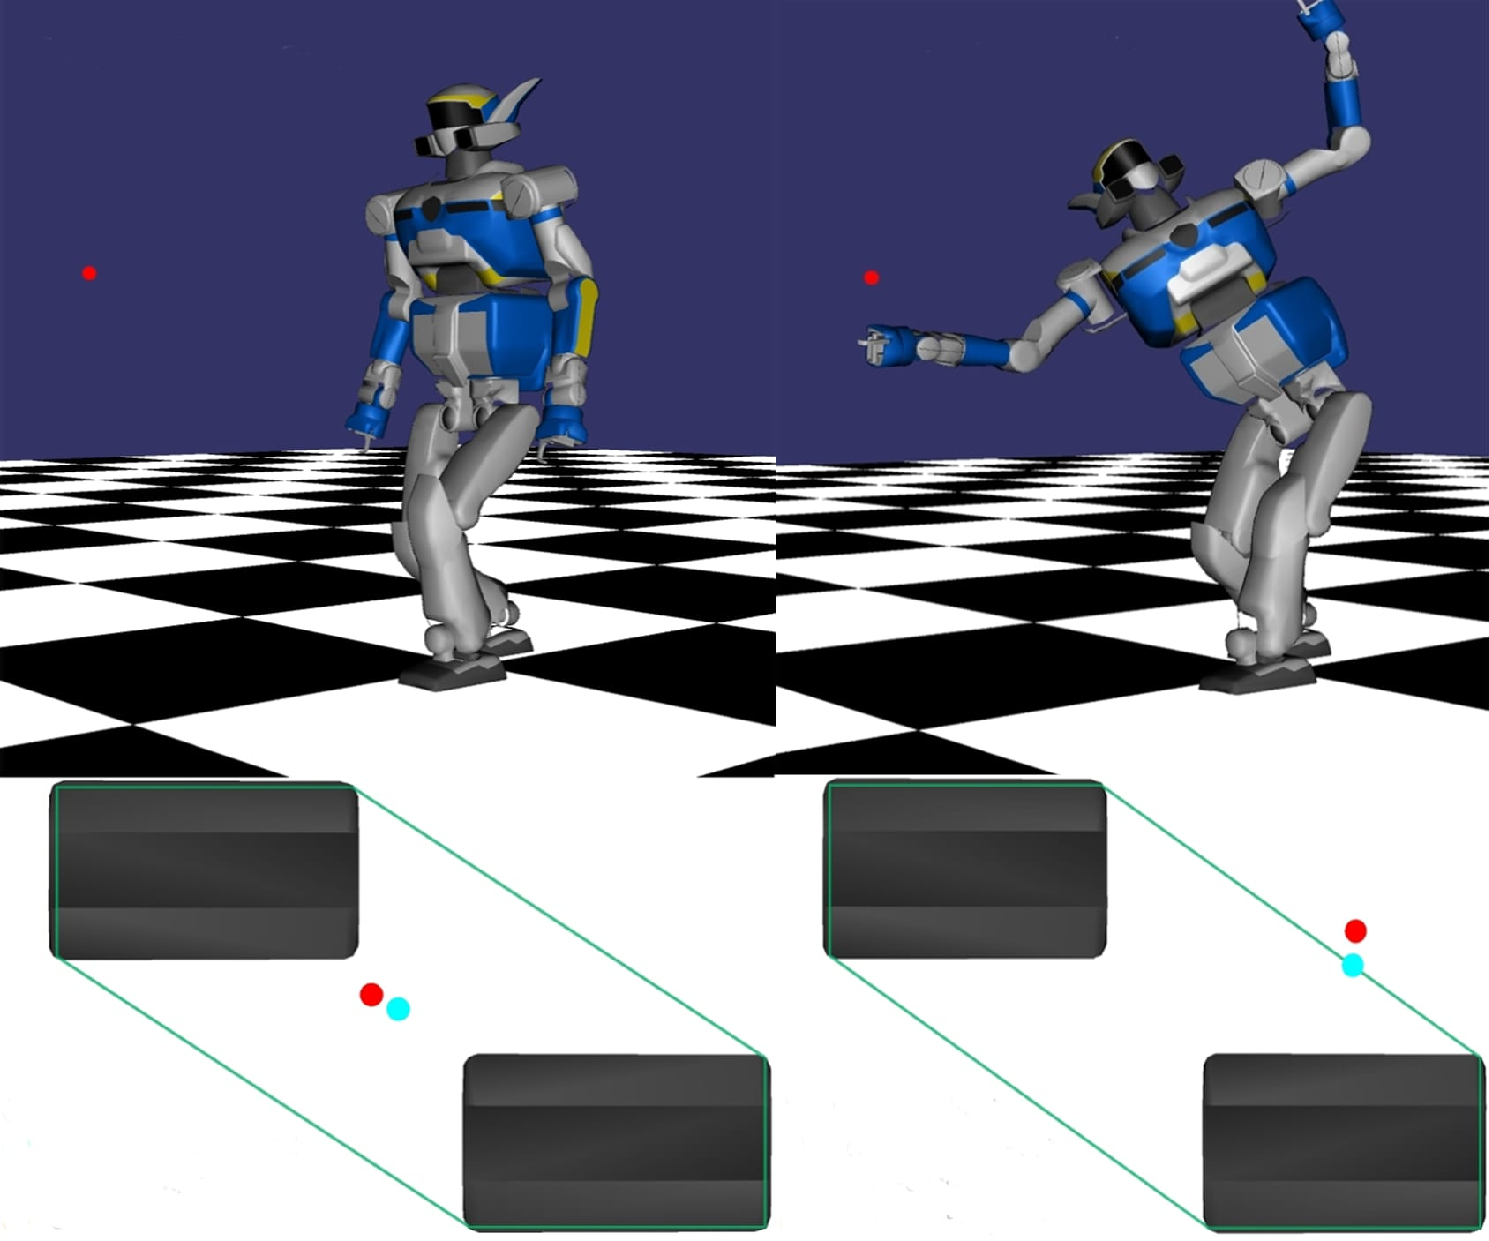
\includegraphics[scale=0.4]{rc_inertial_params/classic_merge.pdf}}\quad
\end{subfigure}
\begin{subfigure}
[Robust control illustrating the robot right end effector reaching close to the goal without losing balance]{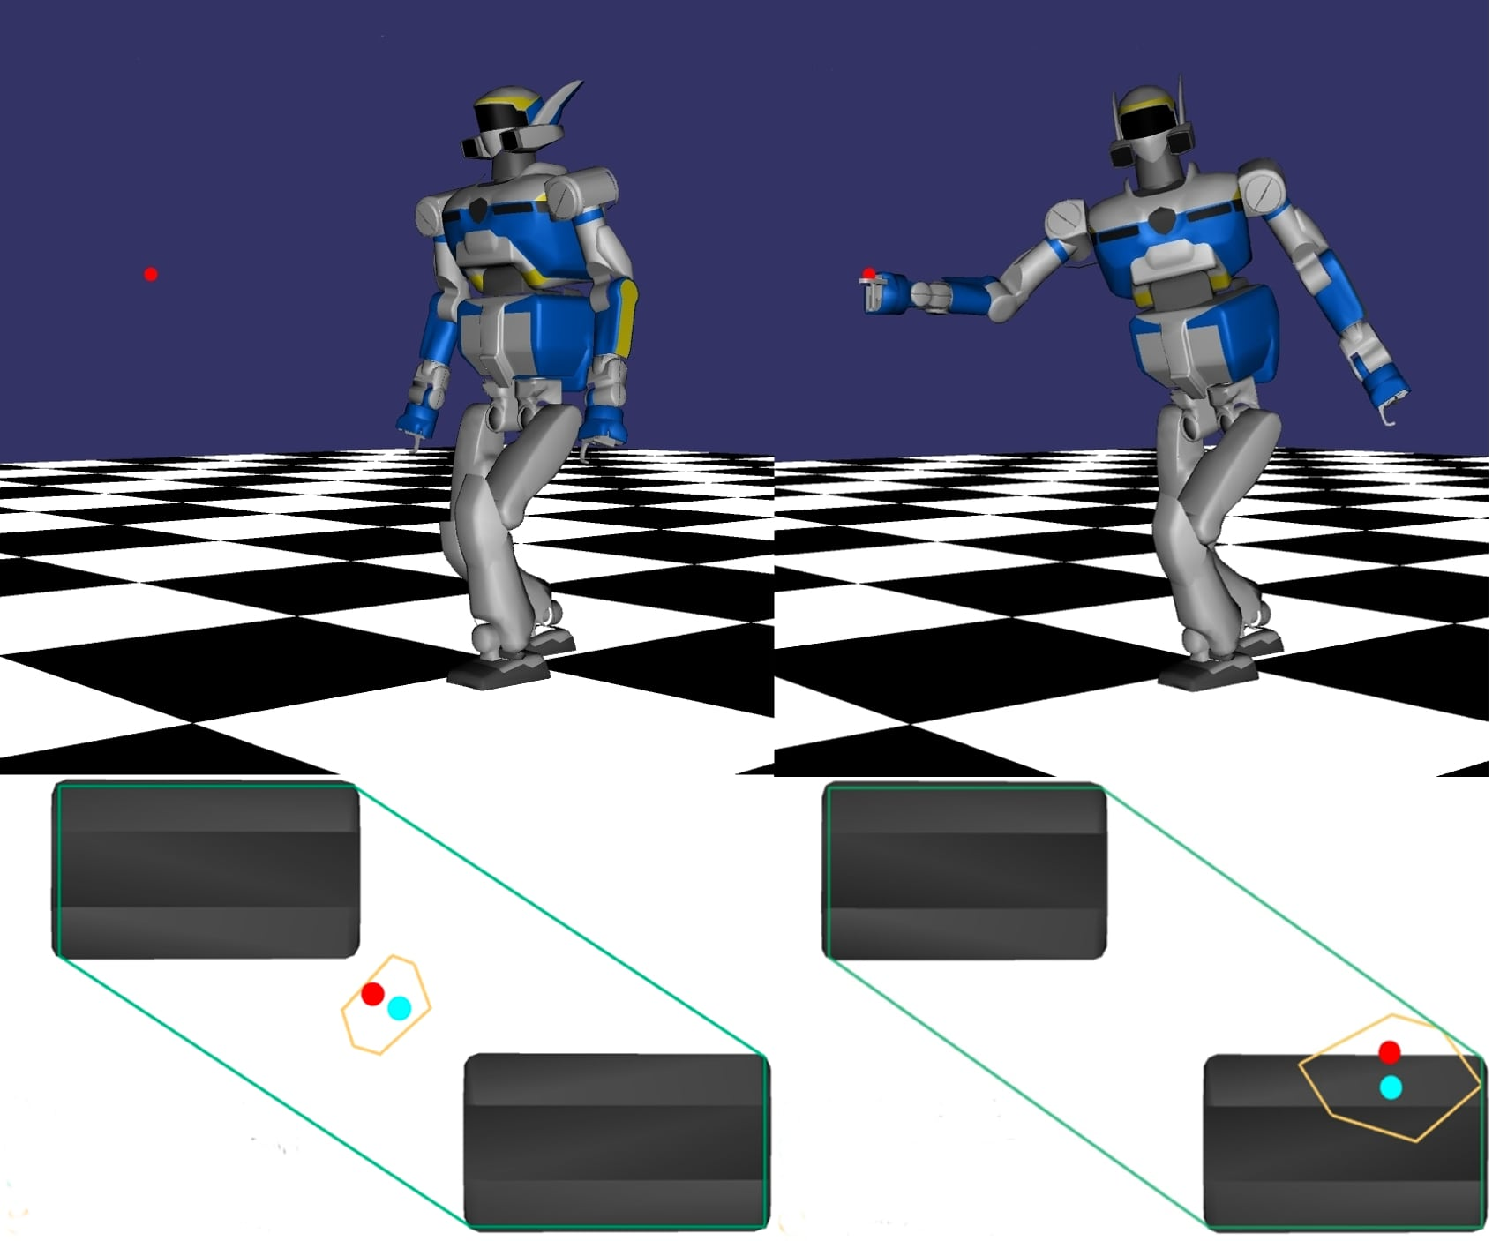
\includegraphics[scale=0.4]{rc_inertial_params/robust_merge.pdf}}\quad
\end{subfigure}\\
 \tikzcircle{3pt}  \footnotesize Real Capture Point \tikzcircle[turquoise, fill=turquoise]{3pt} Estimated Capture Point   \tikzcircle[green, fill=green]{3pt} Support Polygon   \tikzcircle[yellow, fill=yellow]{3pt} Capture Point Polytope

\caption{Screenshots of HRP-2 executing Test 1 to reach the ball target with the robust controller.}
\label{fig:control}
\end{figure*}


\begin{table*}[!tbph]
\begin{center}
\caption{Results of Test 1. For each controller we show the number of falls (Falls), the average time to complete the motion (Task Time) and the average distance of the end-effector to the target at the end of the motion (Task Error).}
\begin{tabular}{ |l|l|l|l|l|l|l|l| }
\hline
\multicolumn{2}{|c|}{Uncertainties}&\multicolumn{3}{|c|}{Classic Controller}&\multicolumn{3}{|c|}{Robust Controller}\\
\hline Max Mass & Max CoM &{Falls}& Task &{Task} & Falls & Task& Task  \\
Error & Error & & Time   &  Error & &  Time & Error\\ 
{[\%]} & [mm] & [\%]  &  [s]  &  [mm]  & [\%]  &  [s] & [mm]\\ 
\hline
% 10 & 12.5& 35& 6.22&4& 1& 5.26& 5\\
% 10 & 25  & 31 & 6.30&  5& 0& 7.32& 12\\
% 10 & 50  & 43 & 4.49 & 70 & 0 & 4.66 & 110\\
% 30 & 50  & 43 & 4.48 & 70 & 0 & 4.68 & 110\\
% 30 & 100 & 40 & 5.44 & 30 & 4 & 5.81 & 80 \\
10 & 10 & 31 & 4.4 & 49 & 3 & 4.5 & 60\\
10 & 20 & 33 & 4.3 & 52 & 1 & 4.5 & 69 \\
10 & 40 & 45 & 4.3 & 55 & 3 & 4.7 & 102\\ 
20 & 10 & 38 & 4.2 & 49 & 11 & 4.5 & 77\\
20 & 20 & 49 & 4.5 & 51 & 9 & 4.55 & 103 \\
20 & 40 & 45 & 4.5 & 59 & 14 & 4.72 & 122 \\
\hline
\end{tabular}
\label{tab:test1}
\end{center}
\end{table*}
\subsection{Test 1}
In this test we set the right end-effector target far in front of the robot.
Fig.~\ref{fig:control}  shows some screen shots of the simulations.
To reach the target the robot must move its CoM (and hence also its capture point) close to the boundaries of its support polygon. 
Table~\ref{tab:test1} presents the results. 
Regardless of the magnitude of the inertial parameter errors, the robust controller managed to prevent the robot from falling almost always, while with the  standard controller the robot fell more than 30\% of the times.
However, since the target was far away from the robot, the robust controller did not manage to reach it because that would have required violating the robust balance constraints.
\begin{table*}[!h]
\begin{center}
\caption{Results of Test 2. For each controller we show the number of falls (Falls), the average time to complete the motion (Task Time) and the average distance of the end-effector to the target at the end of the motion (Task Error).}
\begin{tabular}{ |l|l|l|l|l|l|l|l| }
\hline Max Mass & Max CoM &{Falls}& Task &{Task} & Falls & Task& Task  \\
Error & Error & & Time   &  Error & &  Time & Error\\ 
{[\%]} & [mm] & [\%]  &  [s]  &  [mm]  & [\%]  &  [s] & [mm]\\ 
\hline
% 10 & 12.5 & 59 & 3.64& 0 & 5 & 3.06& 0\\
% 10 & 25.0 & 42 & 3.40 & 0.18 & 4 & 2.94 & 0.12 \\
10 & 10 & 29 & 3.94 & 2 & 0 & 3.4 & 2 \\
10 & 20 & 35 & 3.4 & 2 & 2 & 3.0 & 2 \\
10 & 40 & 42 & 3.86 & 4 & 0 & 2.6 & 4 \\
20 & 10 & 43 & 3.6 & 3 & 0 & 2.8 & 4 \\
20 & 20 & 45 & 3.5 & 3 & 0 & 2.5 & 4 \\
20 & 40 & 45 & 3.0 & 5 & 0 & 2.1 & 5 \\

\hline
\end{tabular}
\label{tab:test2}
\end{center}
\end{table*}
\subsection{Test 2}
In this test we moved the right end-effector target closer to the robot, so that HRP-2 can reach it without moving its CoM close to the support polygon boundaries.
However, we increased the desired speed of reaching (by increasing the gains of the reaching task).
This affected the velocity of the CoM, which in turns affected the capture point, making it reach the boundaries of the support polygon.
The difference with respect to Test 1 is that in this case also the robust controller can reach the target.
Table~\ref{tab:test2} summarizes the results.

Similarly to Test 1, the classic controller leads the robot to a fall in more than 30\% of the cases.
However, contrary to Test 1, this time the robust controller also manages to reach the target, because it is located closer to the robot.
This test shows that being robust does not necessarily implies that we have to sacrifice performance.



%!TEX root =  ../root.tex
\section{Conclusions}
\label{sec:conclusions}
This chapter presented a novel optimization-based inverse-dynamics controller that can balance a legged robot despite bounded uncertainties in its inertial parameters. The controller is based on the state-or-the-art control framework Task-Space Inverse Dynamics. In particular, this work is based on the capture-point inequalities~\cite{Ramos2014a}, which can be included in the controller formulation to ensure the balance of the robot on a level ground. We extended these capture-point inequalities to be robust to bounded uncertainties in the inertial parameters of the robot. The resulting optimization problem is still a Quadratic Program with the same number of variables and inequalities. Moreover, the time required for the additional computation of the robust controller is negligible in this context (i.e. a few microseconds).

We tested the robust controller in simulations with the HRP-2 robot, trying to reach a target position with its right end-effector while balancing. We performed several batches of 100 simulations each, introducing different errors in the inertial parameters and varying the position of the target position and the required speed of motion. Comparisons against a classic TSID controller have shown impressive improvements in terms of fall prevention.

\subsection{Future Work}
In the derivation of the robust controller we saw that the inertial parameters appear in different terms of the optimization problem.
In this preliminary work we focused only on how the uncertainties affect the CoM position.
We believe it should be possible to extend this analysis to the other terms in the capture-point inequalities: CoM velocity, CoM altitude, CoM Jacobian and its time derivative. 
Extending it also to the mass matrix and the bias forces is an interesting future direction, but it seems more challenging because of nonlinearities.

Another issue of the presented approach is that it is rather conservative. As we saw in Test 1, this can lead to poor performance, which can be unacceptable on a real system. Modeling uncertainties with probability distributions (rather than with polytopes) may lead to a less conservative behavior of the system, and it is thus an interesting future direction. In our previous work~\cite{DelPrete2015b} we presented another robust controller, which was robust to joint-torque tracking errors.Integrating the two controllers together seems to be feasible and it would provide robustness to both kinds of uncertainties. In this preliminary work we focused on simulations to validate the controller formulation and to test it with different parameter errors. Of course, we plan also to test the generated movements on the real HRP-2 robot, to quantify how much it can benefit from this robustness.

